\subsection{Finite Element Analysis - Heated Rods - Chapter 31}

Let's re-investigate the heat conduction equation we encountered in
the finite difference methods Section \ref{s:heat1D}. The rod is
discretized in the normal fashion into 5 nodes where the endpoint
temperature values are known as shown in the figure below.

\begin{figure}[H]
  \begin{center}
    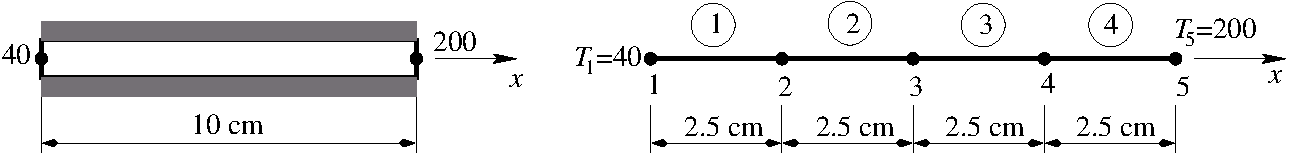
\includegraphics[height=0.1\textwidth,width=0.7\textwidth]{Graphics/L07_F3.pdf}
  \end{center}
\caption{{\bf 1-D Heat Rod for Finite Element Analysis}}\label{f:heatconduction}
\end{figure}

If the body obey's Fourier's law 

\begin{equation}
q = -k \frac{dT}{dx}
\end{equation}

If $k$ is a constant

\beq
k\frac{d^2T}{dx^2} + Q(x) = 0
\eeq

where $Q(x)=dq(x)/dx$ is an internal uniform heat source. 

\begin{enumerate}

\item {\bf Analytic Solution with Q(x) = 0}

The easiest finite element solution is the direct method as has been
done with bars and trusses. This method only applies to $Q(x)=0$. such that 

\beq
\frac{d^2T}{dx^2} = 0
\eeq

To solve the equation the equation above is integrated twice to yield

\beq
T(x) = c_1 x + c_2
\eeq

The boundary conditions are then used to solve for the coefficients
$c_1$ and $c_2$. 

\beq
\begin{matrix}
T(x=0) = T_1 = c_2 = 40 \\
T(x=10) = T_2 = c_1 (10) + 40 = 200 \rightarrow c_1 = 16
\end{matrix}
\eeq

Thus the analytical solution is 

\beq\label{e:heat_rod_direct}
T(x) = 16x+40
\eeq

\item {\bf Direct Method Solution}

Although this equation can be solved for explicitly it is a good
problem to do for its simplicity. Again the question is
to determine the temperature at the nodes in the rod. First let's
examine one element where

\beq\label{e:weighted}
T(x) = N_1T_1 + N_2T_2
\eeq

In this fashion

\beq
\frac{dT}{dx} = T^{'} = \frac{T_2-T_1}{x_2-x_1}
\eeq

which was derived in the previous section. This leads to the heat flux
at node 1 equal to the following.

\beq
q_1 = -k\frac{T_2-T_1}{x_2-x_1} = -kT^{'}
\eeq

In the finite element bar example subject to an axial load, the forces applied
to the beam are equal and opposite. Here similar constraints are
imposed such that $q_1 = -q_2$. This implies that the heat flux
flowing out of 1 bar is equal to the heat flux flowing into 2. Thus,

\beq
q_2 = kT^{'} = k\frac{T_2-T_1}{x_2-x_1}
\eeq

Writing this in matrix form yields the element matrix equation  

\beq
\frac{-k}{x_2-x_1} \begin{bmatrix} -1 & 1 \\ 1 &
  -1 \end{bmatrix} \begin{Bmatrix} T_1 \\ T_2 \end{Bmatrix}
= k \begin{Bmatrix} -T^{'} \\ T^{'} \end{Bmatrix}
\eeq

Dividing out the thermal coefficient $k$, distributing the minus sign
and noting that $T^{'}$ at node 1 is $T^{'}=T^{'}_1$ and $T^{'}=T^{'}_2$ at
node 2 yields the following element matrix.

\beq\label{e:fea_rod_matrix}
\frac{1}{x_2-x_1} \begin{bmatrix} 1 & -1 \\ -1 &
  1 \end{bmatrix} \begin{Bmatrix} T_1 \\ T_2 \end{Bmatrix}
= \begin{Bmatrix} -T^{'}_1 \\ T^{'}_2 \end{Bmatrix}
\eeq

At this point the solution is the same as a bar subject to axial
loads. 

\item {\bf Heat Conduction Bar Example}

Let's now solve the heat conduction problem for the rod in Figure
\ref{f:heatconduction}. First let's write the element stiffness matrix
for elements 1-4. Note that there are 5 nodes and 4 elements where
$x_2-x_1 = \Delta x = 2.5$.

\beq
\begin{bmatrix} 0.4 & -0.4 \\ -0.4 &
  0.4 \end{bmatrix} \begin{Bmatrix} 40 \\ T_2 \end{Bmatrix}
= \begin{Bmatrix} -T^{'}_1 \\ T^{'}_2 \end{Bmatrix}
\eeq

\beq
 \begin{bmatrix} 0.4 & -0.4 \\ -0.4 &
  0.4 \end{bmatrix} \begin{Bmatrix} T_2 \\ T_3 \end{Bmatrix}
= \begin{Bmatrix} -T^{'}_2 \\ T^{'}_3 \end{Bmatrix}
\eeq

\beq
\begin{bmatrix} 0.4 & -0.4 \\ -0.4 &
  0.4 \end{bmatrix} \begin{Bmatrix} T_3 \\ T_4 \end{Bmatrix}
= \begin{Bmatrix} -T^{'}_3 \\ T^{'}_4 \end{Bmatrix}
\eeq

\beq
 \begin{bmatrix} 0.4 & -0.4 \\ -0.4 &
 0.4 \end{bmatrix} \begin{Bmatrix} T_4 \\ 200 \end{Bmatrix}
= \begin{Bmatrix} -T^{'}_4 \\ T^{'}_5 \end{Bmatrix}
\eeq

Just as before this is combined to a full bar element matrix such that

\beq\label{e:fea_rod_matrix_solution}
\begin{bmatrix} 0.4 & -0.4 & 0 & 0 & 0 \\
-0.4 & 0.8 & -0.4 & 0 & 0 \\
0 & -0.4 & 0.8 & -0.4 & 0 \\
0 & 0 & -0.4 & 0.8 & -0.4 \\
0 & 0 & 0 & -0.4 & 0.4 \end{bmatrix}\begin{Bmatrix} 40
  \\ T_2 \\ T_3 \\ T_4 \\ 200 \end{Bmatrix} = \begin{Bmatrix} -T_1^{'}
  \\ 0 \\ 0\\0\\T_5^{'}\end{Bmatrix}
\eeq

Notice that the internal heat flux was canceled due to equal and
opposite reactions. The formulation of these equations led to two
unknowns being introduced. That is, $T_1^{'}$ and $T_5^{'}$ are now
unknowns. The equations must be rearranged to yield the following
equations. 

\beq
\begin{bmatrix} 1 & -0.4 & 0 & 0 & 0 \\
0 & 0.8 & -0.4 & 0 & 0 \\
0 & -0.4 & 0.8 & -0.4 & 0 \\
0 & 0 & -0.4 & 0.8 & 0 \\
0 & 0 & 0 & -0.4 & -1 \end{bmatrix}\begin{Bmatrix} T_1^{'}
  \\ T_2 \\ T_3 \\ T_4 \\ T_5^{'} \end{Bmatrix} = \begin{Bmatrix} -16
  \\ 16 \\ 0\\80\\-80\end{Bmatrix}
\eeq

This equation is of the form $A\vec{x} = \vec{b}$ which can be solved
explicitly for the temperature. The figure below shows the result of
the analytic solution from equation \ref{e:heat_rod_direct} and the
numerical solution from above.

\begin{figure}[H]
  \begin{center}
    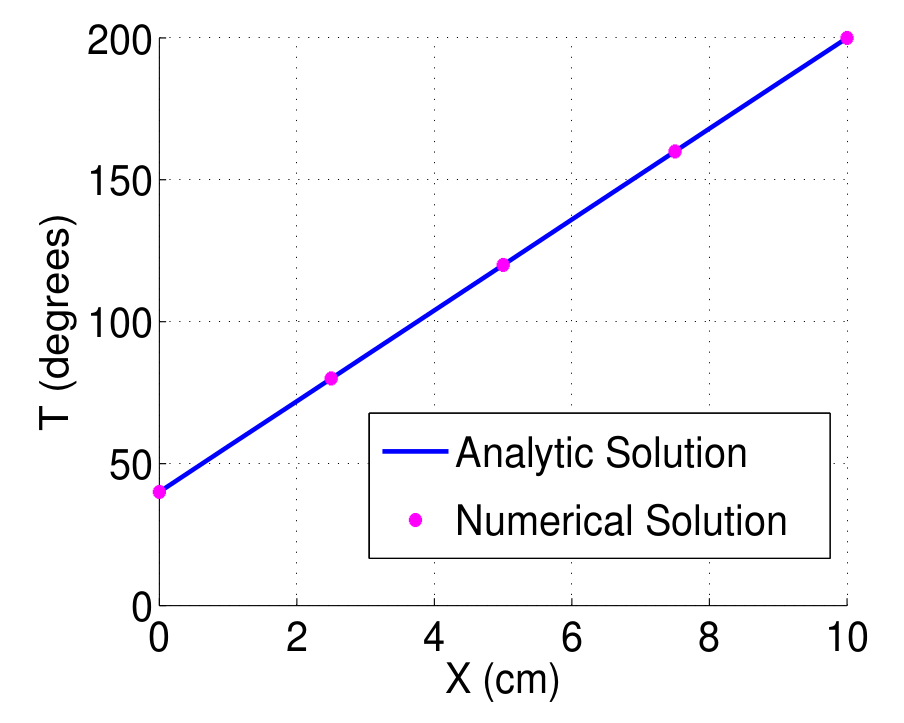
\includegraphics[height=0.4\textwidth,width=0.5\textwidth]{Graphics/Heat_Rod_Direct}
  \end{center}
\end{figure}

\item {\bf Method of Weighted Residuals}

The direct method above works well if $Q(x) = 0$; however, it is it's
major shortcoming. Let's re-investigate the same problem above however
setting $Q(x)/k = 10$. This equation can again be solved analytically
since

\beq
\frac{d^2T}{dx^2} = -10
\eeq

which leads to the temperature solution shown below where the boundary
conditions $T(0) = 40$ and $T(10) = 200$ are used to solve for the
undetermined coefficients. 

\beq
T(x) = -5 x^2 + 66 x + 40
\eeq

In order to solve this using finite element analysis the heat equation
is written as

\beq
\frac{d^2T}{dx^2} + f(x) = 0
\eeq

Then using equation \ref{e:weighted} which is an approximate solution
leads to 

\beq
\frac{d^2\tilde{T}}{dx^2} + f(x) = R
\eeq

where R is a residual since the equation is only an approximation. The
method of weighted residuals then requires

\beq
\int\limits_D R W_i dD = 0
\eeq

where $W_i$ are weights force the integrand to zero. D is the entire
control volume. For this case the control volume is the length of the
rod and the weighted functions are the interpolation functions
$N_i$. This method is called Galerkin's method.

\beq
\int\limits_D R N_i dD = 0 = \int\limits_{x_1}^{x_2}
\left[\frac{d^2\tilde{T}}{dx^2} + f(x)\right] N_i~dx = 0
\eeq

which can also be written as

\beq\label{e:mwr1}
\int\limits_{x_1}^{x_2}\frac{d^2\tilde{T}}{dx^2}N_i~dx= -\int\limits_{x_1}^{x_2} f(x) N_i dx
\eeq

The integrand on the left can be evaluated using integration by parts

\beq\label{e:mwr2}
\int\limits_{x_1}^{x_2}\frac{d^2\tilde{T}}{dx^2}N_i~dx = N_i \frac{d\tilde{T}}{dx} \Big|_{x_1}^{x_2}-\int\limits_{x_1}^{x_2}\frac{d\tilde{T}}{dx}\frac{dN_i}{dx}dx
\eeq

The first term on the right hand side can be evaluated to yield 

\beq\label{e:mwr3}
N_1 \frac{d\tilde{T}}{dx} \Big|_{x_1}^{x_2} =
N_1(x_2)T_2^{'} - N_1(x_1)T_1^{'}
\eeq

where $i=1$. Remember that $N_1(x_2)=0$ and $N_1(x_1)=1$ so

\beq
N_1 \frac{d\tilde{T}}{dx} \Big|_{x_1}^{x_2} = -T_1^{'}
\eeq

Similarly with $i=2$ 

\beq
N_2 \frac{d\tilde{T}}{dx} \Big|_{x_1}^{x_2} = T_2^{'}
\eeq

using equations \ref{e:mwr1} through \ref{e:mwr3} leads to the
following two equations for $i=1$ and $i=2$ 

\beq
\int\limits_{x_1}^{x_2}\frac{d\tilde{T}}{dx}\frac{dN_1}{dx}dx =
-T_1^{'} + \int\limits_{x_1}^{x_2} f(x) N_1 dx
\eeq

\beq
\int\limits_{x_1}^{x_2}\frac{d\tilde{T}}{dx}\frac{dN_2}{dx}dx =
T_2^{'} + \int\limits_{x_1}^{x_2} f(x) N_2 dx
\eeq

The first terms in the left-hand side are simple to evaluate using the
shape functions. 

\beq
\int\limits_{x_1}^{x_2}\frac{d\tilde{T}}{dx}\frac{dN_1}{dx}dx = -\frac{T_2-T_1}{x_2-x_1}
\eeq

\beq
\int\limits_{x_1}^{x_2}\frac{d\tilde{T}}{dx}\frac{dN_2}{dx}dx = \frac{T_2-T_1}{x_2-x_1}
\eeq

If the equation above is written in matrix form the equation is
identical to the element matrix written in \ref{e:fea_rod_matrix}
except there is an external forcing function added that must be
evaluated. 

\beq
\frac{1}{x_2-x_1} \begin{bmatrix} 1 & -1 \\ -1 &
  1 \end{bmatrix} \begin{Bmatrix} T_1 \\ T_2 \end{Bmatrix}
= \begin{Bmatrix} -T^{'}_1 \\ T^{'}_2 \end{Bmatrix}
+ \begin{Bmatrix} \int\limits_{x_1}^{x_2} f(x) N_1 dx
  \\ \int\limits_{x_1}^{x_2} f(x) N_2 dx \end{Bmatrix}
\eeq

The solution to the example with $Q(x)/L = 10$ is solved in the same
fashion as before only the forcing functions must be evaluated for
each element. Just as before this is done for all 4 elements to yield
8 equations. The equations are then stacked together to yield only 5
equations as shown in the equations below. The equations are again
identical to \ref{e:fea_rod_matrix_solution} only the forcing function
adds a bit extra to the equation.

\beq
\begin{bmatrix} 0.4 & -0.4 & 0 & 0 & 0 \\
-0.4 & 0.8 & -0.4 & 0 & 0 \\
0 & -0.4 & 0.8 & -0.4 & 0 \\
0 & 0 & -0.4 & 0.8 & -0.4 \\
0 & 0 & 0 & -0.4 & 0.4 \end{bmatrix}\begin{Bmatrix} 40
  \\ T_2 \\ T_3 \\ T_4 \\ 200 \end{Bmatrix} = \begin{Bmatrix} -T_1^{'}
  + 12.5
  \\ 25 \\ 25 \\ 25 \\ T_5^{'} + 12.5 \end{Bmatrix}
\eeq

Just as before the equations are altered to solve for the introduced
unknowns $T_1^{'}$ and $T_2^{'}$ which leads to the equation

\beq
\begin{bmatrix} 1 & -0.4 & 0 & 0 & 0 \\
0 & 0.8 & -0.4 & 0 & 0 \\
0 & -0.4 & 0.8 & -0.4 & 0 \\
0 & 0 & -0.4 & 0.8 & 0 \\
0 & 0 & 0 & -0.4 & 1 \end{bmatrix}\begin{Bmatrix} T_1^{'}
  \\ T_2 \\ T_3 \\ T_4 \\ T_5^{'} \end{Bmatrix} = \begin{Bmatrix} -3.5
  \\ 41 \\ 25 \\ 105 \\ -67.5 \end{Bmatrix}
\eeq

Again, this can be solved on any numerical computer and the solution
is shown in the figure below.

\begin{figure}[H]
  \begin{center}
    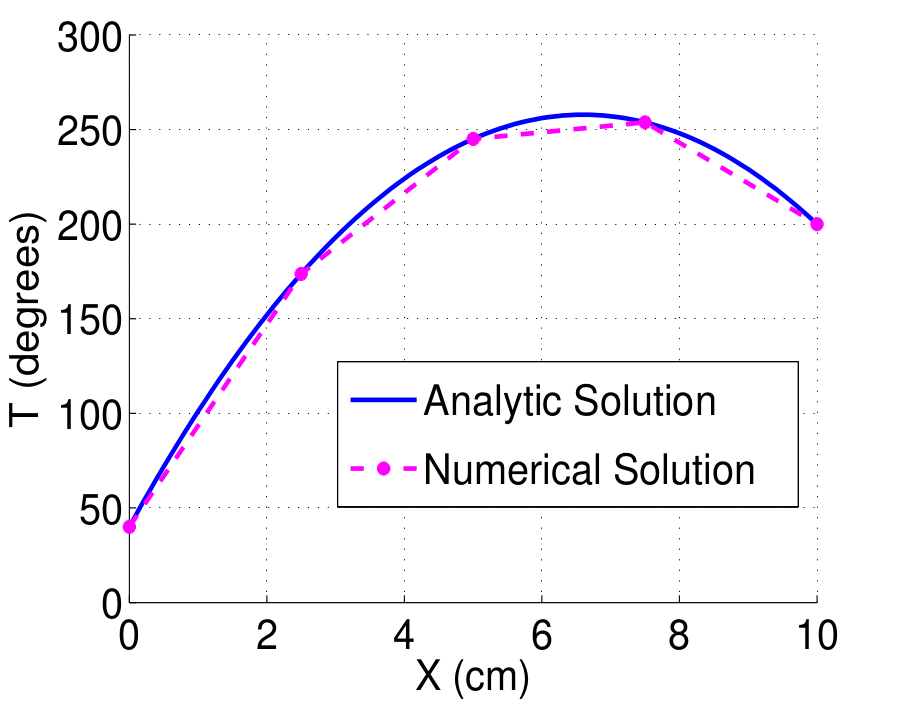
\includegraphics[height=0.4\textwidth,width=0.5\textwidth]{Graphics/Heat_Rod_FEA}
  \end{center}
\end{figure}

Notice however that the solution is not quite exact since the shape
functions are linear. Obviously there are solutions where the shape
functions are quadratic but these are beyond the scope of this text.

\end{enumerate}
    


